\definecolor{lightblue}{HTML}{CFE2F3}
\definecolor{lightgreen}{HTML}{8AB8A7}
\definecolor{lighttan}{HTML}{f6f0e8}
\definecolor{tan}{HTML}{e8d8c3}

\newcommand\gpcolor{tan}
\newcommand\aqccolor{lighttan!50}
\newcommand\evalcolor{gray!30}

\begin{tikzpicture}
  [
    node distance=1.5cm,
    every node/.style={font=\large},
    align=center,
    background rectangle/.style={fill=white},
    show background rectangle
  ]
      \tikzset{
        >={Latex[width=2mm,length=2mm]},
        base/.style = {rectangle, rounded corners, draw=black,
                       minimum width=1cm, minimum height=1cm,
                       text centered},
        block/.style = {base, minimum width=2.5cm, minimum height=1.5cm, inner sep=3mm},
        bbstyle/.style = {block, fill=black, text=white},
        opstyle/.style = {block, fill=white},
        surrogatestyle/.style = {block, fill=\gpcolor},
        evalstyle/.style = {block, fill=\evalcolor},
        acqstyle/.style = {block, fill=\aqccolor},
        taskstyle/.style = {block, fill=white},
        iterationstyle/.style = {base, fill=none, draw=gray, dashed, minimum width=4cm},
    }
    \pgfdeclarelayer{iterationlayer}
    \pgfsetlayers{background,iterationlayer,main}

    \node (acqs) [acqstyle, inner sep=5mm, text width=115mm] {{\Large Acquisition Functions}\\[12pt]\begin{enumerate}[leftmargin=1.5em]
        \item \textbf{Uncertainty exploration}
            \begin{flalign*}
                \phantom{\mu'(}\vec{x}'_1 = \begin{cases}
                    \vec{x}' \leftarrow \displaystyle\argmax_{\vec{x} \in \mathcal{X}} \hat{\sigma}(\vec{x})p(\vec{x})^{1/\alpha t} & \text{if } \tau = 0\\
                    \vec{x}' \sim \big( \hat{\sigma}(\vec{x})p(\vec{x})^{1/\alpha t} \big)^{1/\tau} & \text{otherwise}
                \end{cases}&&
            \end{flalign*}
        \item \textbf{Boundary refinement}
            \begin{flalign*}
                \mu'(\vec{x}) &= \hat{f}(\vec{x})(1 - \hat{f}(\vec{x}))&&\\
                \vec{x}'_2 &= \begin{cases}
                    \vec{x}' \leftarrow \displaystyle\argmax_{\vec{x} \in \mathcal{X}} \bigl(\mu'(\vec{x}) + \lambda\hat{\sigma}(\vec{x})\bigr)p(\vec{x})^{1/\alpha t} & \text{if } \tau = 0\\
                    \vec{x}' \sim \big( \bigl(\mu'(\vec{x}) + \lambda\hat{\sigma}(\vec{x})\bigr)p(\vec{x})^{1/\alpha t} \big)^{1/\tau} & \text{otherwise}
                \end{cases}&&
            \end{flalign*}
        \item \textbf{Failure region sampling}
            \begin{flalign*}
                \phantom{'}\hat{h}(\vec{x}) &= \hat{f}(\vec{x}) + \lambda\hat{\sigma}(x)&&\\
                \phantom{'}\hat{g}(\vec{x}) &= \mathds{1}\bigl\{\hat{h}(\vec{x}) \ge 0.5\bigl\}&&\\
                \vec{x}'_3 &= \begin{cases}
                    \vec{x}' \sim \hat{h}(\vec{x}) & \text{if } \hat{g}(\vec{x}) = 0,\, \forall \vec{x} \in \mathcal{X} \\
                    \vec{x}' \sim \hat{g}(\vec{x})\hat{h}(\vec{x})p(\vec{x}) & \text{otherwise}
                \end{cases}&&
            \end{flalign*}
    \end{enumerate}};
    \node (surrogate) [surrogatestyle, above left=-10mm and 8mm of acqs] {Probabilistic\\Surrogate Model\\[6pt]$\hat{f}(\vec{x})$,  $\hat{\sigma}(\vec{x})$};
    \node (eval) [evalstyle, below=113mm of surrogate] {System Evaluations\\[6pt]$\vec{y} = \bigl\{ f(\vec{x}') \mid \vec{x}' \in [\vec{x}'_1, \vec{x}'_2, \vec{x}'_3] \bigr\}$};

    \begin{pgfonlayer}{iterationlayer}
        \path let \p1=(surrogate.north west), \p2=(acqs.south east) in node (iteration) [fit={($(\x1,\y1)+(-1.5cm,0.25cm)$) ($(\x2,\y2)+(0.3cm,-26mm)$)}, iterationstyle]{};
        \node at ($(iteration.north west)+(2cm,4mm)$) [text=gray!50!black] {iteration $t \in [1,\ldots,T]$};
    \end{pgfonlayer}

    \node (blackbox) [bbstyle, above left=12.5mm and 12mm of iteration.west, anchor=east] {Black-box System\\$f(\vec{x})$};
    \node (opmodel) [opstyle, below=10mm of blackbox.south, anchor=north] {Operational Model\\$p(\vec{x})$};

    \node (pfail) [taskstyle, right=12mm of iteration.south east, anchor=south west] {
        \textsc{Failure Probability Estimation}\\
        {(using importance sampling)}\\
        \phantom{}\\
        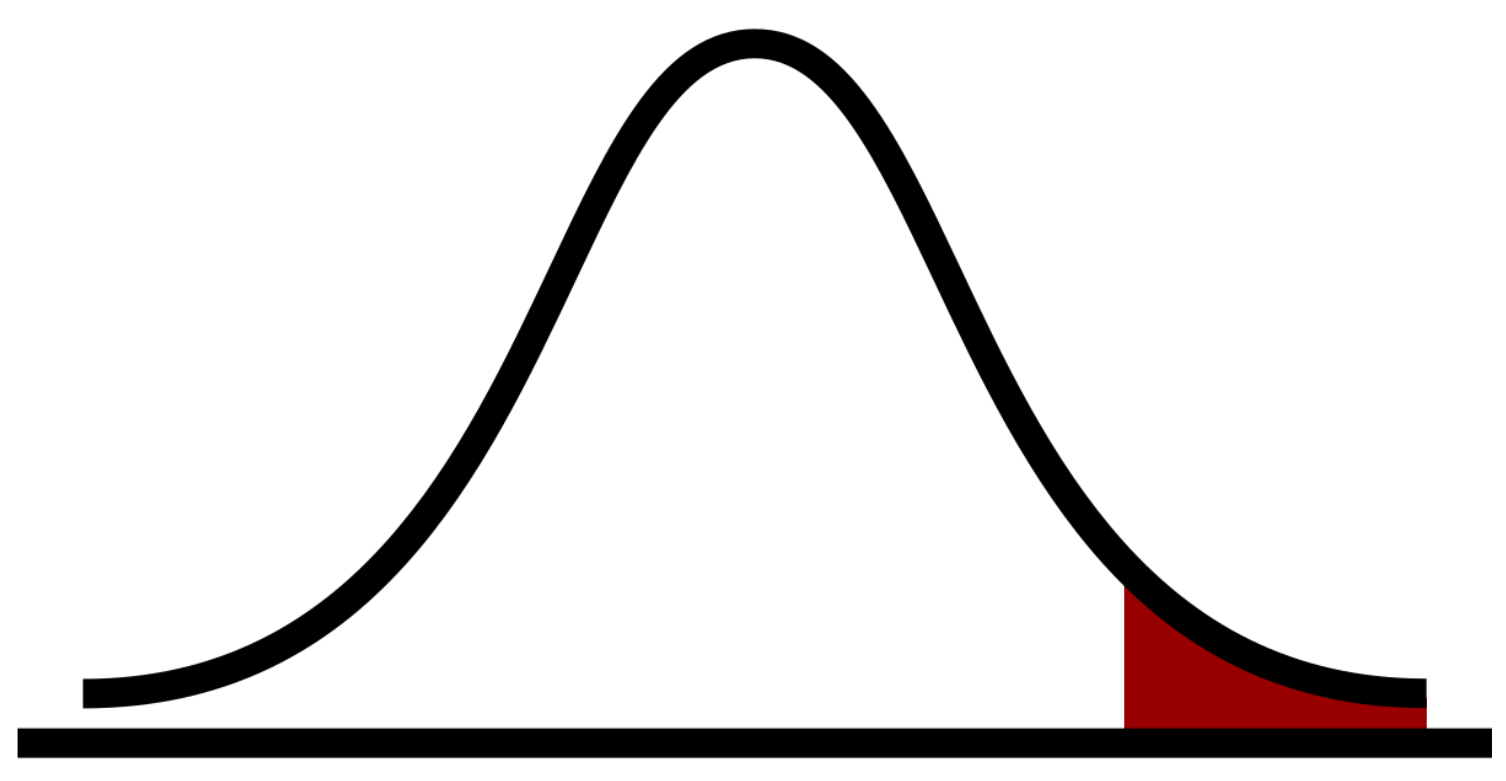
\includegraphics[width=4cm]{diagrams/bsv/pfail-distribution.png}\\
        \phantom{}\\
        $\hat{p}_\text{fail} \approx\begin{cases}
            \frac{1}{n} \sum_{i=1}^n \frac{p(\vec{x}_i)}{q(\vec{x}_i)} \mathds{1}\left\{\hat{f}(\vec{x}_i) \ge 0.5 \right\} \\
            \left(\sum_{i=1}^n \vec{W}_i \vec{Y}_i\right) / \sum_{i=1}^n \vec{W}_i
        \end{cases}$
    };
    \node (falsification) [taskstyle, above=73mm of pfail.north, anchor=south] {\textsc{Falsification}\\[6pt]$\vec{X}_\text{fail} = \big\{\vec{x}_i \mid \vec{x}_i \in \vec{X},\, y_i \in \vec{Y},\, \mathds{1}\{y_i\}\big\}$};
    \node (mlfa) [taskstyle, below=5mm of falsification.south, anchor=north] {\textsc{Most-likely Failure Analysis}\\[6pt]$\displaystyle\vec{x}^* = \argmax_{\substack{\vec{x}_i \in \vec{X}\\y_i \in \vec{Y}}} p(\vec{x}_i)\mathds{1}\{y_i\}$};

    \draw[->] (blackbox.east) -| ++(4.4mm,0) |- ($(iteration.west)+(0,2.5mm)$);
    \draw[->] (opmodel.east) -| ++(2.875mm,0) |- ($(iteration.west)+(0,-2.5mm)$);

    \draw[->] (eval.north) -- (surrogate.south) node[pos=0.5, above, fill=white]{re-fit surrogate model\\given observations $\vec{y}$};
    \draw[->] ($(surrogate.east)+(0mm,6mm)$) -| (acqs.north);
    \draw[->] ($(acqs.south)+(-2cm,0mm)$) |- ($(eval.east)+(0mm,4mm)$) node[pos=0.58, above] {$\vec{x}'_1$};
    \draw[->] (acqs.south) |- (eval.east) node[pos=0.54, above] {$\vec{x}'_2$};
    \draw[->] ($(acqs.south)+(2cm,0mm)$) |- ($(eval.east)+(0mm,-4mm)$) node[pos=0.53, above] {$\vec{x}'_3$};

    \draw[->] ($(iteration.east)+(0mm,23mm)$) -| ++(3.5mm,-0) |- (falsification.west);
    \draw[->] ($(iteration.east)+(0mm,14mm)$) -| ++(7mm,-0) |- (mlfa.west) node[pos=0, yshift=2mm, right] {\ sampled points $\vec{X}$ and observations $\vec{Y}$};
    \draw[->] ($(iteration.east)+(0mm,3mm)$) -| (pfail.north) node[pos=0.43, above] {final surrogate model $\hat{f}(\vec{x}), \hat{\sigma}(\vec{x})$};
\end{tikzpicture}
